\chapter{Análise de Concorrentes}

Auditamos soluções que existem atualmente no mercado e, ao verificar
as aplicações existentes, conclui-se que há intersecções nas funções
dentre os aplicativos analisados. As funções mais básicas, como
gerenciamento de itens e gerenciamento de listas, estão presentes em
todos, tendo em vista que são essenciais em qualquer aplicativo de
lista. Outras funções básicas que deveriam ser incluídas em qualquer
aplicação de lista, como gerenciamento de categorias e
compartilhamento de listas, não estão presentes em todos os
aplicativos analisados.

Contudo, as divergências ficam claras quando analisamos o mecanismo
das aplicações, entre elas destacam-se o Mealime e o Cozi Family
Organizer que, apesar de serem voltados para as compras, cumprem
também outras funcionalidades. O Mealime, cujo foco é o planejamento
de refeições, e o Cozi Family Organizer, cujo foco é o planejamento
familiar, deixam a desejar nas funções relacionadas às compras.

Entre os outros aplicativos analisados, é perceptível que não possuem
todas as funcionalidades propostas nesse documento, principalmente
quando se trata de compartilhamento de listas, uma vez que cada
software lida de modo diferente diante dessa feature. O SoftList, por
exemplo, permite o compartilhamento de lista, porém não é capaz de ser
gerenciada por mais de um usuário, sendo apenas importada para o
usuário no qual a lista está sendo compartilhada.

Ao analisar os aplicativos mais populares da categoria, constatamos
que o Out Of Milk, Bring! e o OurGroceries, que são destaques na área,
não se propõem a exibir análise estatística das compras do usuário e
nem manter um histórico do que foi comprado. \DIFaddbegin \DIFadd{A tabela \ref{tbl:concorrentes}
permite visualizar melhor as diferenças entre os concorrentes.
}\DIFaddend 

\pagebreak

\section{Tabela de Comparação}

\DIFdelbegin %DIFDELCMD < \begin{figure}[h!]
%DIFDELCMD < 	\centering
%DIFDELCMD < 	%%%
%DIF < 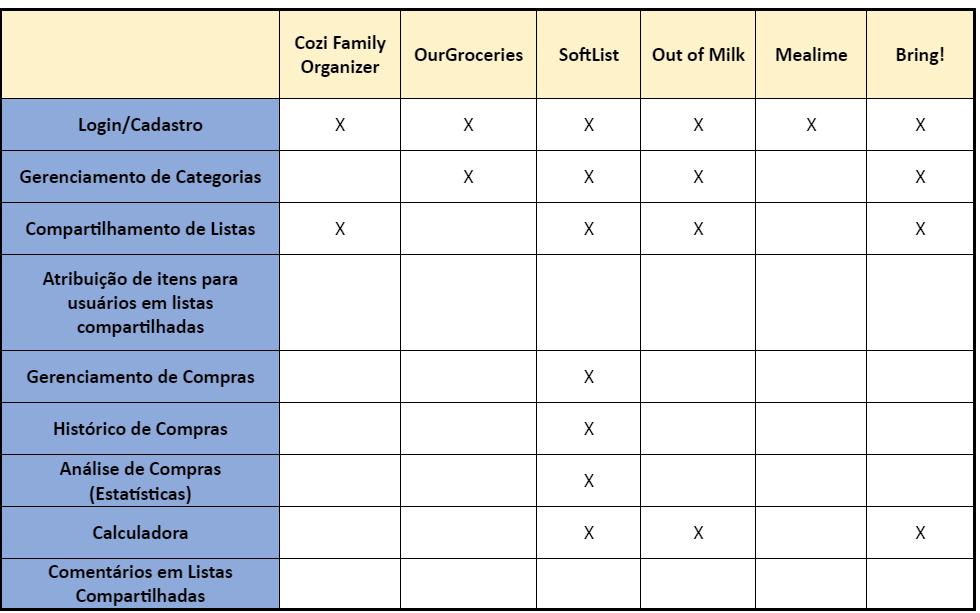
\includegraphics[scale=0.65]{./imagens/tabela_comparativa.png}
	%DIFDELCMD < 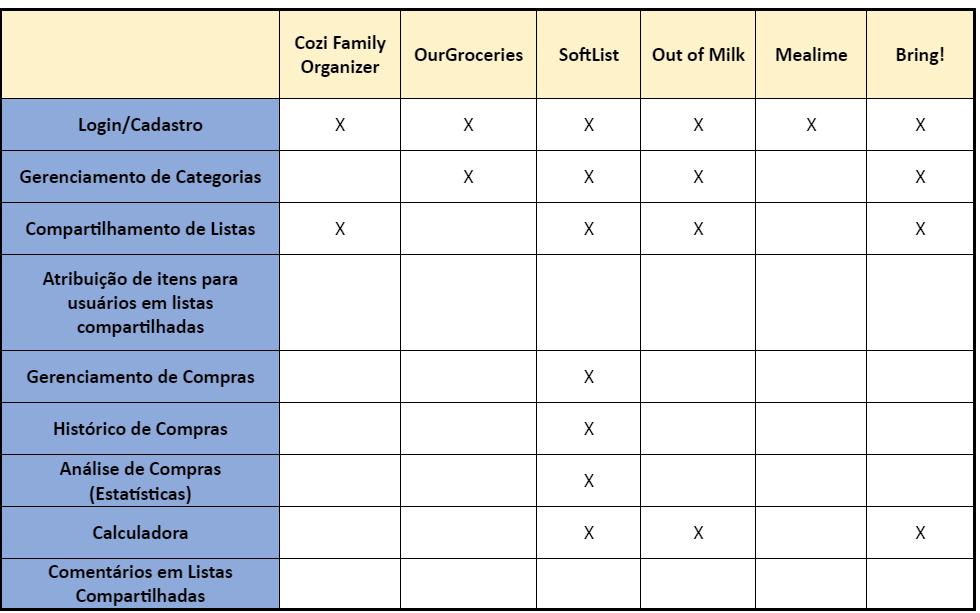
\includegraphics[width=.8\textwidth,height=\textheight,keepaspectratio]{./imagens/tabela_comparativa.png} 
%DIFDELCMD < 	%%%
\DIFdelendFL \DIFaddbeginFL \label{tbl:concorrentes}
\begin{center}
  \resizebox{\columnwidth}{!}{%
    \begin{tabular}{lccccccc}
      \hline
      & Cozi Family Organizer & OurGroceries & Softlist & Out of Milk & Mealime
      & Bring & Lixt\\
      \hline
      Login/Cadastro & x & x & x & x & x & x & x\\
      \hline
      Categorias &  & x & x & x &  & x & x\\
      \hline
      Compartilhamento de listas & x &  & x & x &  & x & x\\
      \hline
      Atribuição de itens &  &  &  &  &  &  & x\\
      \hline
      Gerenciamento de compras &  &  & x &  &  &  & x\\
      \hline
      Historico de compras &  &  & x &  &  &  & x\\
      \hline
      Análise de compras &  &  & x &  &  &  & x\\
      \hline
      Calculadora &  &  & x & x &  & x & x\\
      \hline
      Comentários &  &  &  &  &  &  & x\\
      \hline
    \end{tabular}
  }
  \DIFaddendFL \caption{\DIFdelbeginFL \DIFdelFL{Comparativo de Concorrentes}\DIFdelendFL \DIFaddbeginFL \DIFaddFL{Tabela \ref{tbl:concorrentes}: Uma comparação dos aplicativos concorrentes.}\DIFaddendFL }
\DIFdelbeginFL %DIFDELCMD < \end{figure}
%DIFDELCMD < 	 %%%
\DIFdelend \DIFaddbegin \end{center}
%DIF > %% Local Variables:
%DIF > %% mode: latex
%DIF > %% TeX-master: "../proposta"
%DIF > %% End:
 \DIFaddend